\chapter{Additional Material}

A usable simulation app is available at  \url{http://statchats.wordpress.com}. These apps are built with Rshiny and are hosted by Rstudio.

\label{AppendixA}
\begin{figure}[!h]
\centering
\begin{subfigure}{.45\textwidth}
  \centering
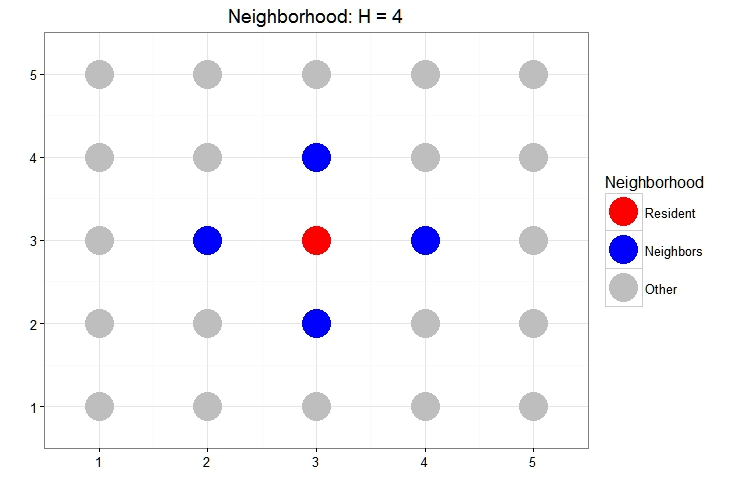
\includegraphics[scale=.33]{figures/H4.jpeg}
\end{subfigure}%
\begin{subfigure}{.45\textwidth}
  \centering
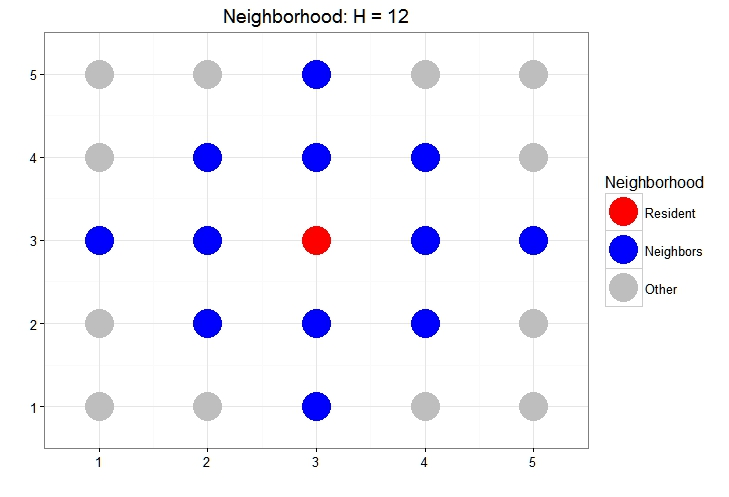
\includegraphics[scale=.33]{figures/H12.jpeg}
\end{subfigure}
\caption[Manhattan Distance]{Manhattan Distance: $d=1$ and $d=2$}
\label{fig:MD}
\end{figure}

\begin{figure}[h!]
\centering
\begin{subfigure}{.5\textwidth}
  \centering
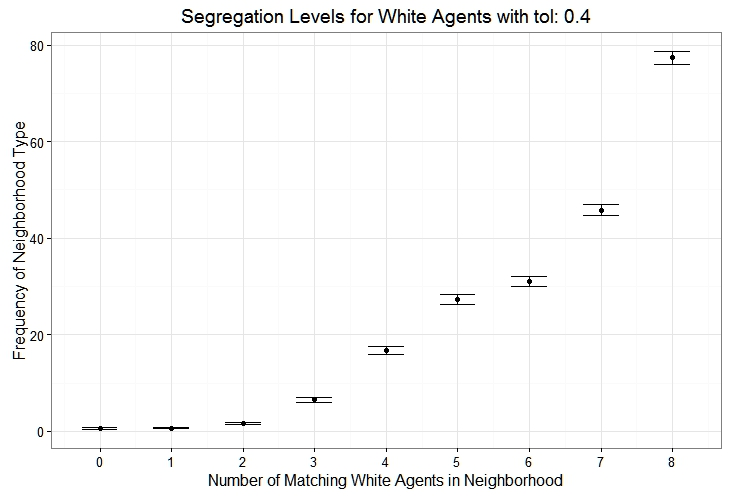
\includegraphics[scale=.35]{figures/2000_4_White.jpeg}
\end{subfigure}%
\begin{subfigure}{.5\textwidth}
  \centering
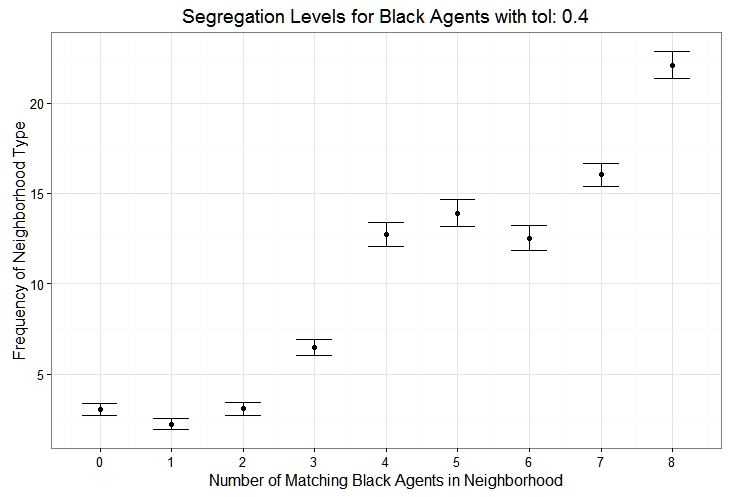
\includegraphics[scale=.35]{figures/2000_4_Black.jpeg}
\end{subfigure}
\hfill \break \hfill \break
\begin{subfigure}{.5\textwidth}
  \centering
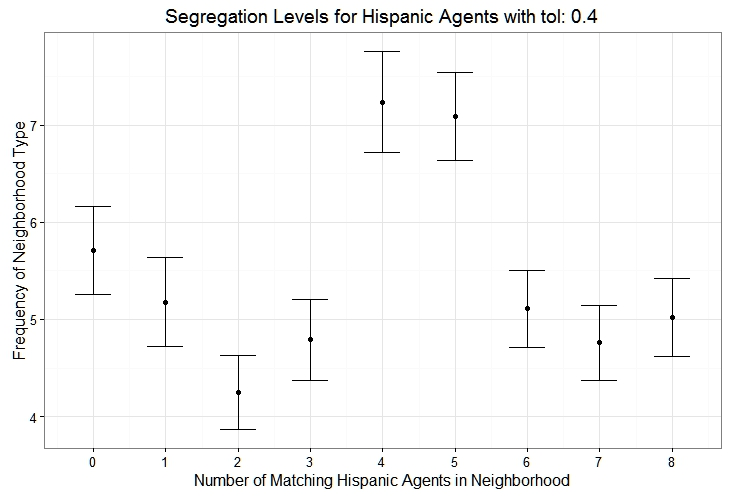
\includegraphics[scale=.35]{figures/2000_4_Hispanic.jpeg}
\end{subfigure}%
\begin{subfigure}{.5\textwidth}
  \centering
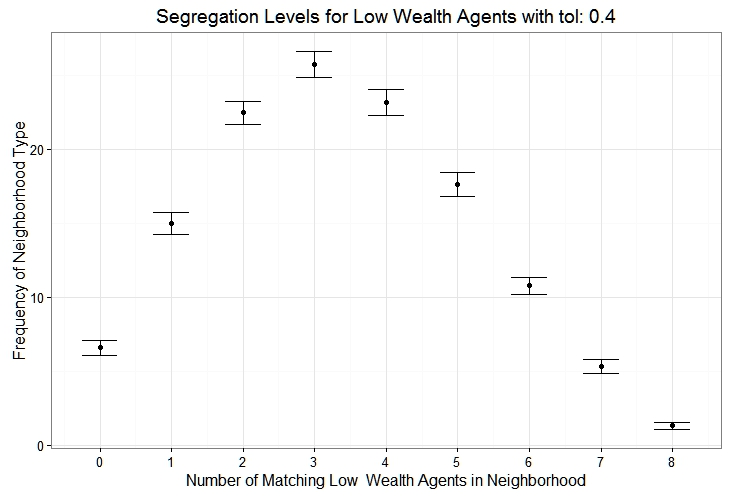
\includegraphics[scale=.35]{figures/2000_4_Low.jpeg}
\end{subfigure}
\hfill \break \hfill \break
\begin{subfigure}{.5\textwidth}
  \centering
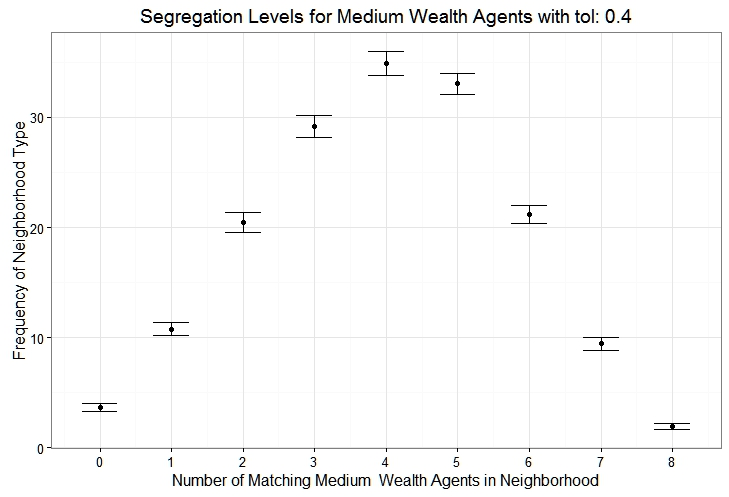
\includegraphics[scale=.35]{figures/2000_4_Med.jpeg}
\end{subfigure}%
\begin{subfigure}{.5\textwidth}
  \centering
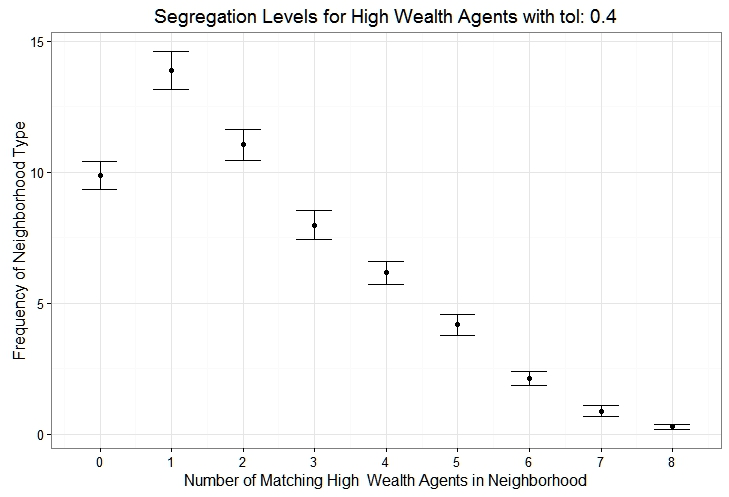
\includegraphics[scale=.35]{figures/2000_4_High.jpeg}
\end{subfigure}
\caption[Simulated Demographics ($\tau = 40\%$); 2000 Chicago]{Histograms of Simulated Demographics ($\tau = 40\%$) in 2000 Chicago}
\end{figure}

\begin{figure}[h!]
\centering
\begin{subfigure}{.5\textwidth}
  \centering
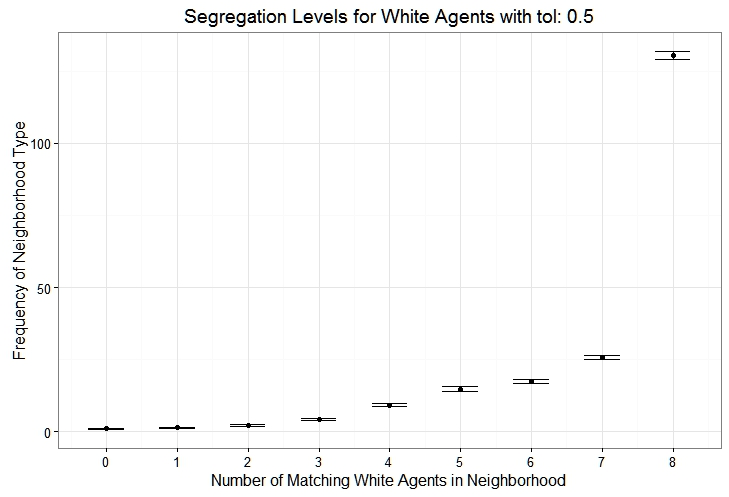
\includegraphics[scale=.35]{figures/2000_5_White.jpeg}
\end{subfigure}%
\begin{subfigure}{.5\textwidth}
  \centering
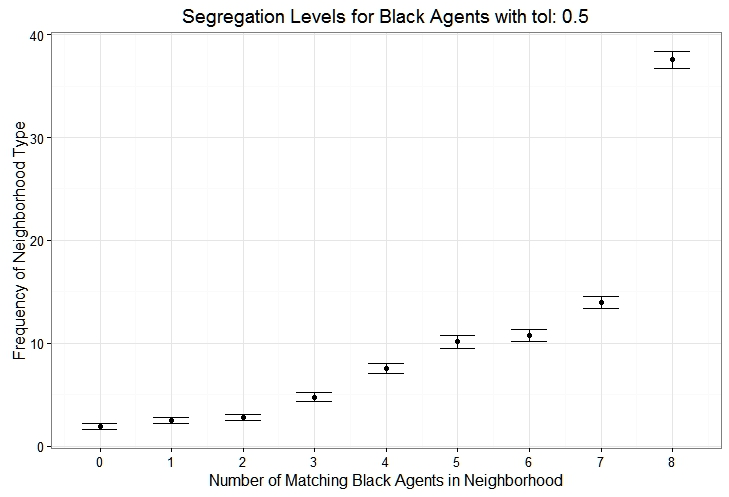
\includegraphics[scale=.35]{figures/2000_5_Black.jpeg}
\end{subfigure}
\hfill \break \hfill \break
\begin{subfigure}{.5\textwidth}
  \centering
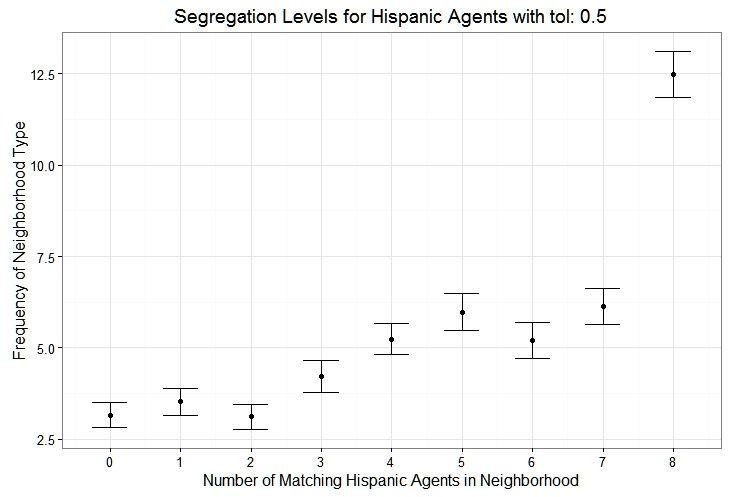
\includegraphics[scale=.35]{figures/2000_5_Hispanic.jpeg}
\end{subfigure}%
\begin{subfigure}{.5\textwidth}
  \centering
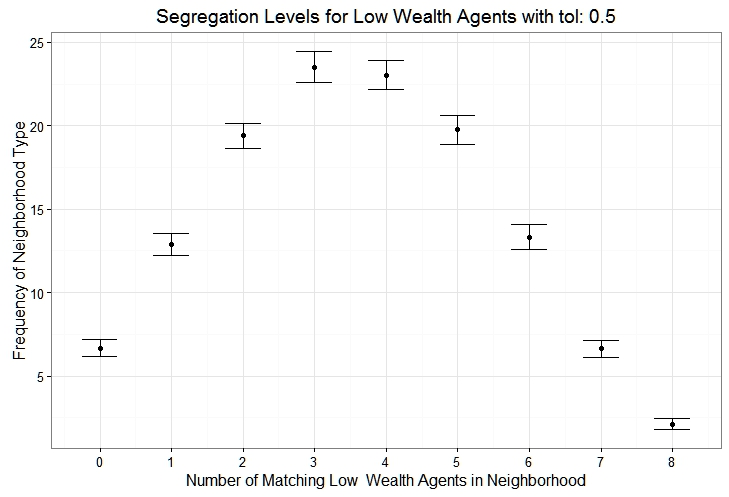
\includegraphics[scale=.35]{figures/2000_5_Low.jpeg}
\end{subfigure}
\hfill \break \hfill \break
\begin{subfigure}{.5\textwidth}
  \centering
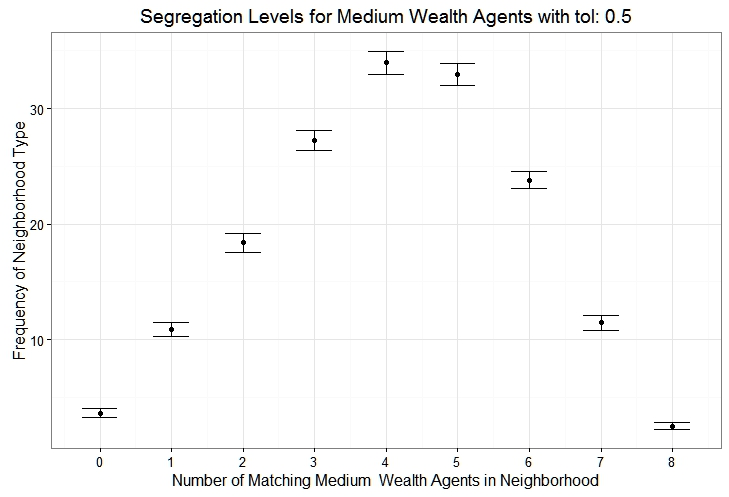
\includegraphics[scale=.35]{figures/2000_5_Med.jpeg}
\end{subfigure}%
\begin{subfigure}{.5\textwidth}
  \centering
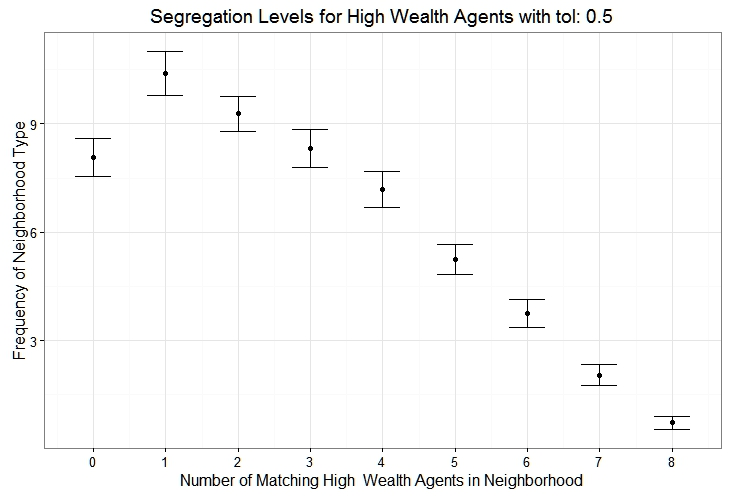
\includegraphics[scale=.35]{figures/2000_5_High.jpeg}
\end{subfigure}
\caption[Simulated Demographics ($\tau = 50\%$); 2000 Chicago]{Histograms of Simulated Demographics ($\tau = 50\%$) in 2000 Chicago}
\end{figure}

\begin{figure}[h!]
\centering
\begin{subfigure}{.5\textwidth}
  \centering
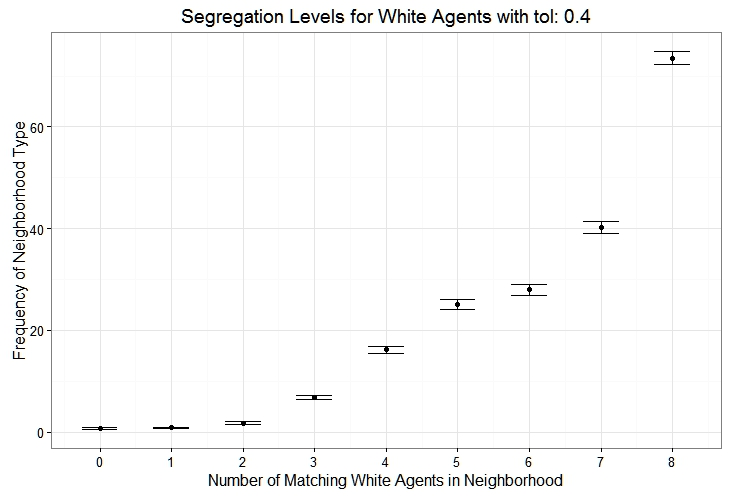
\includegraphics[scale=.35]{figures/2010_4_White.jpeg}
\end{subfigure}%
\begin{subfigure}{.5\textwidth}
  \centering
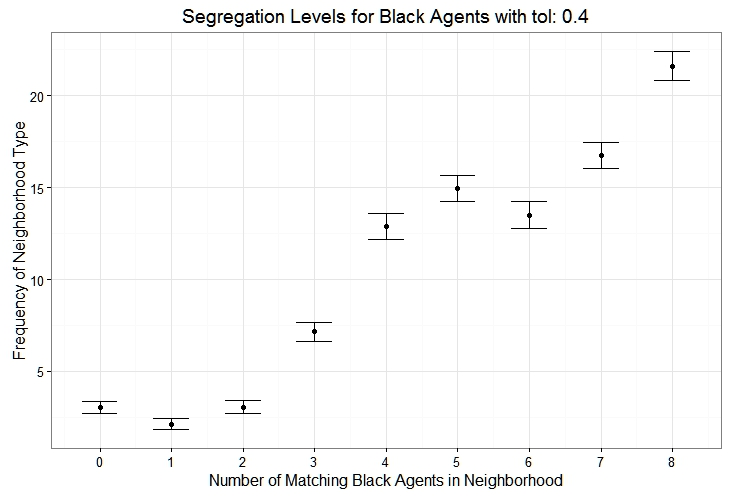
\includegraphics[scale=.35]{figures/2010_4_Black.jpeg}
\end{subfigure}
\hfill \break \hfill \break
\begin{subfigure}{.5\textwidth}
  \centering
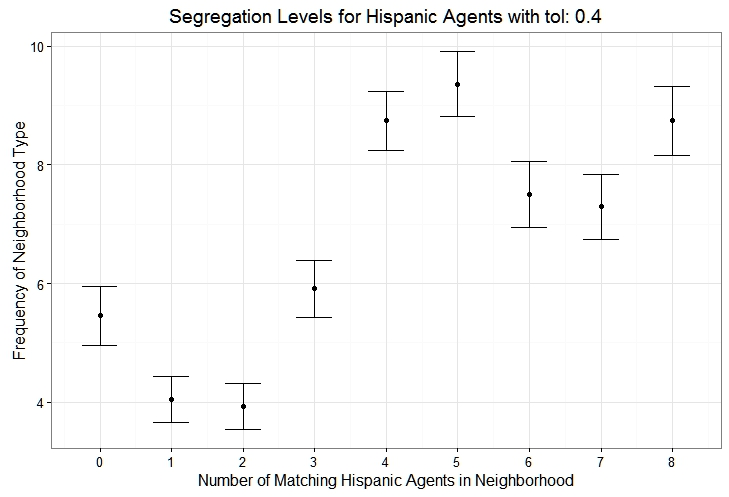
\includegraphics[scale=.35]{figures/2010_4_Hispanic.jpeg}
\end{subfigure}%
\begin{subfigure}{.5\textwidth}
  \centering
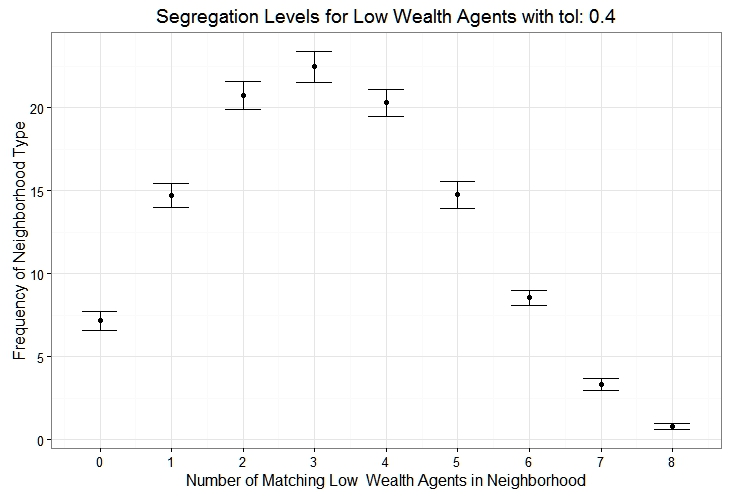
\includegraphics[scale=.35]{figures/2010_4_Low.jpeg}
\end{subfigure}
\hfill \break \hfill \break
\begin{subfigure}{.5\textwidth}
  \centering
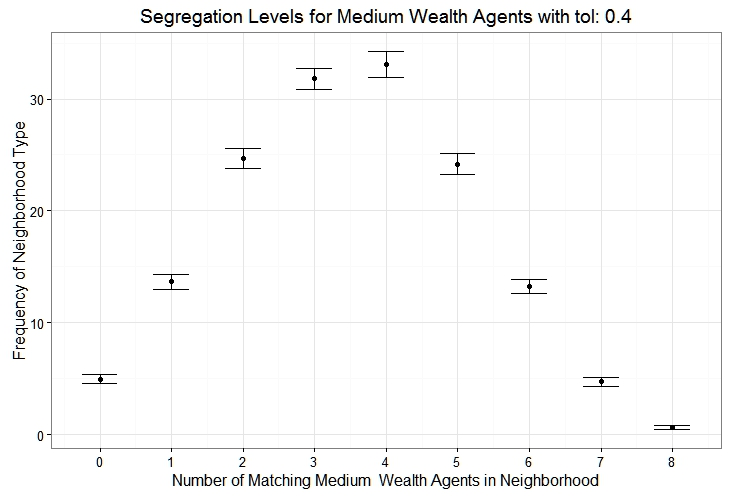
\includegraphics[scale=.35]{figures/2010_4_Med.jpeg}
\end{subfigure}%
\begin{subfigure}{.5\textwidth}
  \centering
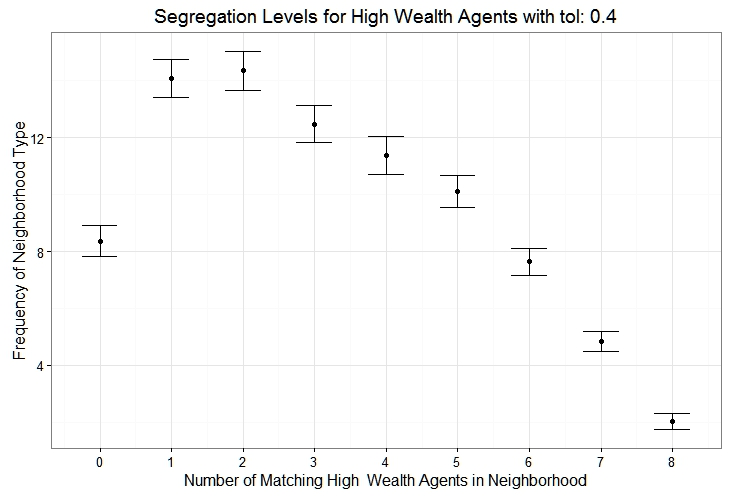
\includegraphics[scale=.35]{figures/2010_4_High.jpeg}
\end{subfigure}
\caption[Simulated Demographics ($\tau = 40\%$); 2010 Chicago]{Histograms of Simulated Demographics ($\tau = 40\%$) in 2010 Chicago}
\end{figure}

\begin{figure}[h!]
\centering
\begin{subfigure}{.5\textwidth}
  \centering
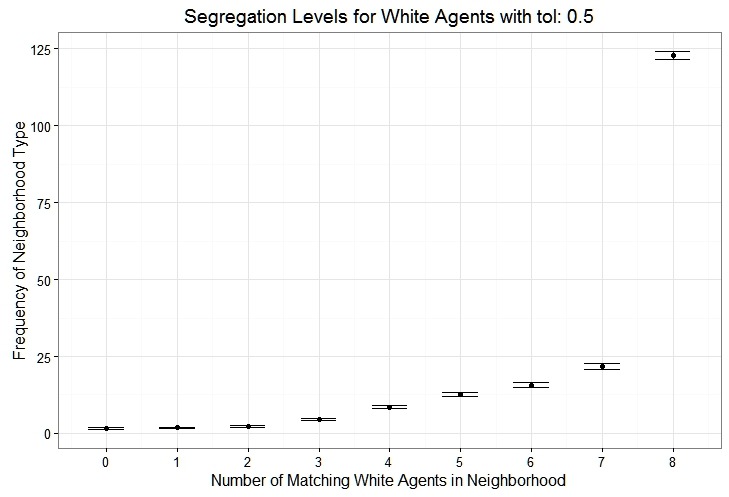
\includegraphics[scale=.35]{figures/2010_5_White.jpeg}
\end{subfigure}%
\begin{subfigure}{.5\textwidth}
  \centering
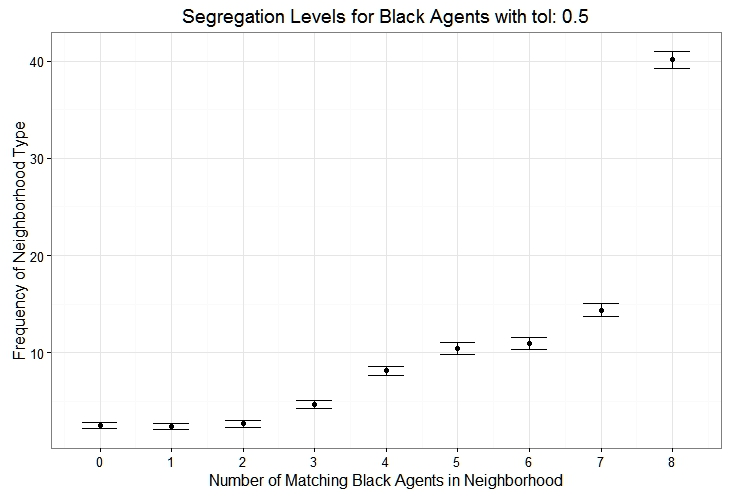
\includegraphics[scale=.35]{figures/2010_5_Black.jpeg}
\end{subfigure}
\hfill \break \hfill \break
\begin{subfigure}{.5\textwidth}
  \centering
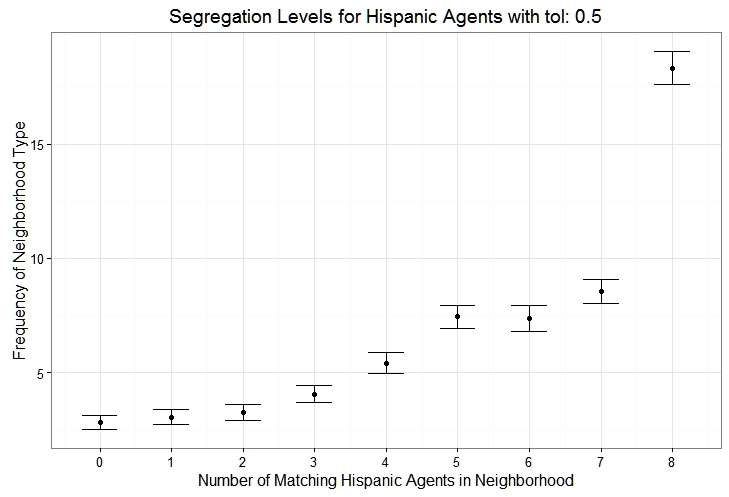
\includegraphics[scale=.35]{figures/2010_5_Hispanic.jpeg}
\end{subfigure}%
\begin{subfigure}{.5\textwidth}
  \centering
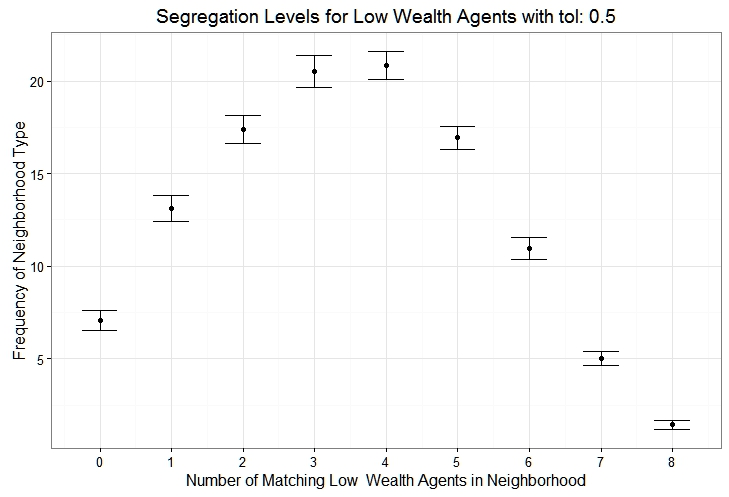
\includegraphics[scale=.35]{figures/2010_5_Low.jpeg}
\end{subfigure}
\hfill \break \hfill \break
\begin{subfigure}{.5\textwidth}
  \centering
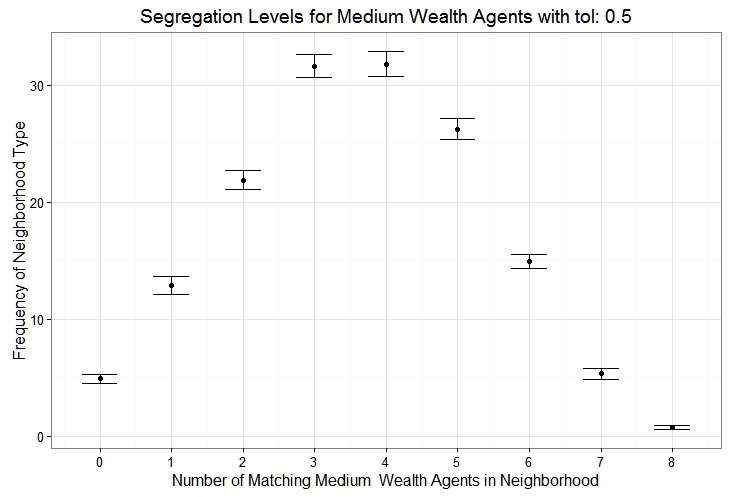
\includegraphics[scale=.35]{figures/2010_5_Med.jpeg}
\end{subfigure}%
\begin{subfigure}{.5\textwidth}
  \centering
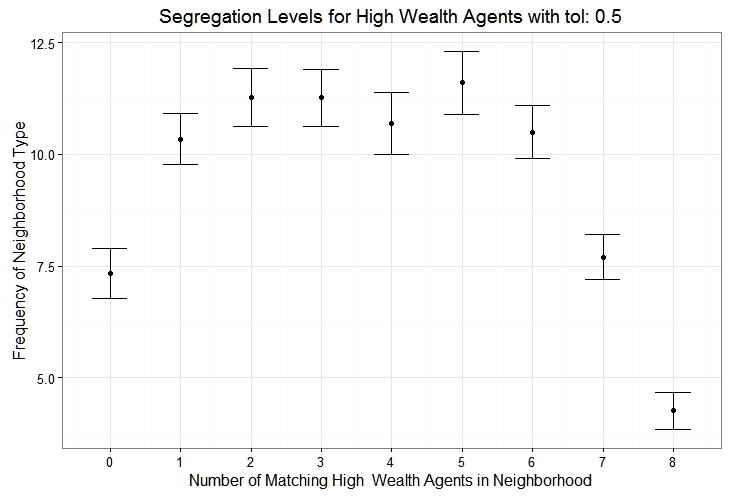
\includegraphics[scale=.35]{figures/2010_5_High.jpeg}
\end{subfigure}
\caption[Simulated Demographics ($\tau = 50\%$); 2010 Chicago]{Histograms of Simulated Demographics ($\tau = 50\%$) in 2010 Chicago}
\end{figure}